\documentclass[border=4pt]{standalone}
\usepackage{amssymb}
\usepackage{tikz}
\usetikzlibrary{arrows.meta,positioning,shapes.geometric,fit,calc,automata,trees}
\usepackage{float}
\usepackage{booktabs}
\usepackage{longtable}
\usepackage{array}
\usepackage[utf8]{inputenc}
\begin{document}

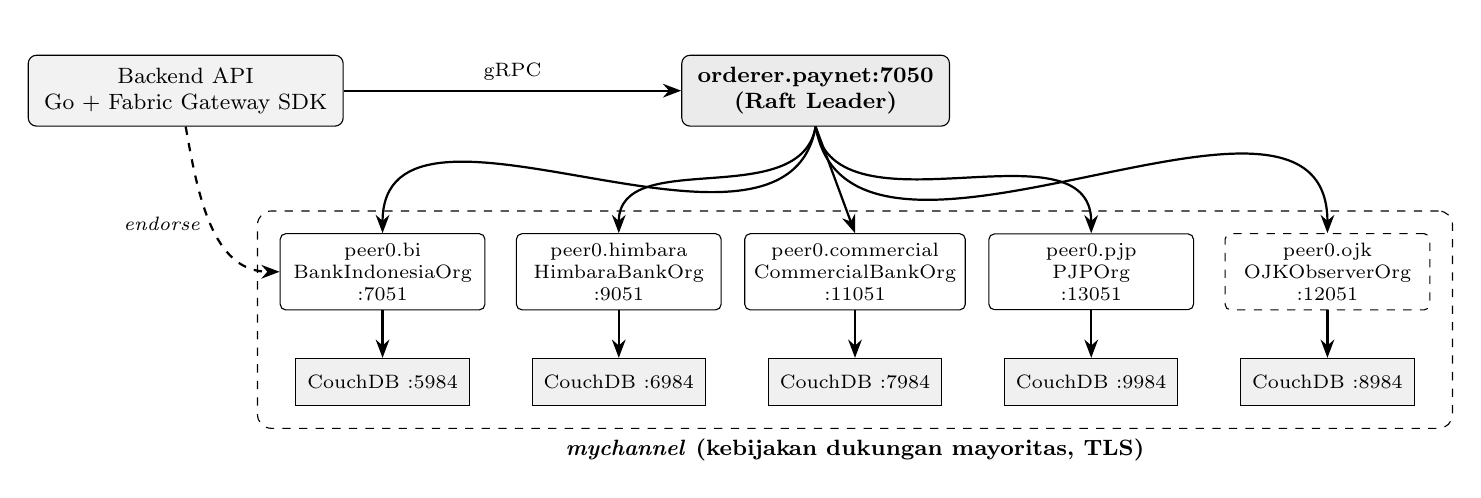
\begin{tikzpicture}[
  peer/.style={draw=black, fill=white, rectangle, rounded corners=2pt,
    minimum width=2.6cm, minimum height=0.9cm, align=center, font=\scriptsize},
  observer/.style={draw=black, dashed, fill=none, rectangle, rounded corners=2pt,
    minimum width=2.6cm, minimum height=0.9cm, align=center, font=\scriptsize},
  cdb/.style={draw=black, fill=gray!12, rectangle,
    minimum width=2.2cm, minimum height=0.6cm, align=center, font=\scriptsize},
  ordnode/.style={draw=black, fill=black!8, rectangle, rounded corners=3pt,
    minimum width=3.4cm, minimum height=0.9cm, align=center, font=\footnotesize\bfseries},
  backend/.style={draw=black, fill=black!5, rectangle, rounded corners=3pt,
    minimum width=4.0cm, minimum height=0.9cm, align=center, font=\footnotesize},
  chanbox/.style={draw=black, dashed, rounded corners=5pt,
    fill=none, inner sep=8pt},
  ar/.style={-{Stealth}, thick},
  gar/.style={-{Stealth}, thick, dashed},
  pathlabel/.style={font=\scriptsize, midway, align=center},
]

%--- Backend + Orderer ---
\node[backend] (be)  at (-2.5, 3.5) {Backend API\\Go + Fabric Gateway SDK};
\node[ordnode] (ord) at ( 5.5, 3.5) {orderer.paynet:7050\\(Raft Leader)};
\draw[ar] (be.east) -- node[pathlabel,above]{gRPC} (ord.west);

%--- Peer nodes ---
\node[peer]     (pbi)  at ( 0.0, 1.2) {peer0.bi\\BankIndonesiaOrg\\:7051};
\node[peer]     (phim) at ( 3.0, 1.2) {peer0.himbara\\HimbaraBankOrg\\:9051};
\node[peer]     (pcom) at ( 6.0, 1.2) {peer0.commercial\\CommercialBankOrg\\:11051};
\node[peer]     (ppjp) at ( 9.0, 1.2) {peer0.pjp\\PJPOrg\\:13051};
\node[observer] (pojk) at (12.0, 1.2) {peer0.ojk\\OJKObserverOrg\\:12051};

%--- Orderer delivers block to all peers ---
\draw[ar] (ord.south) to[out=-100,in=90] (pbi.north);
\draw[ar] (ord.south) to[out=-100,in=90] (phim.north);
\draw[ar] (ord.south) -- (pcom.north);
\draw[ar] (ord.south) to[out=-80,in=90]  (ppjp.north);
\draw[ar] (ord.south) to[out=-80,in=90]  (pojk.north);

%--- Backend gateway to peer0.bi ---
\draw[gar] (be.south) to[out=-80,in=180]
  node[pathlabel,left]{\textit{endorse}} (pbi.west);

%--- CouchDB state databases ---
\node[cdb] (cbi)  at ( 0.0, -0.2) {CouchDB :5984};
\node[cdb] (chim) at ( 3.0, -0.2) {CouchDB :6984};
\node[cdb] (ccom) at ( 6.0, -0.2) {CouchDB :7984};
\node[cdb] (cpjp) at ( 9.0, -0.2) {CouchDB :9984};
\node[cdb] (cojk) at (12.0, -0.2) {CouchDB :8984};

\draw[ar] (pbi)  -- (cbi);
\draw[ar] (phim) -- (chim);
\draw[ar] (pcom) -- (ccom);
\draw[ar] (ppjp) -- (cpjp);
\draw[ar] (pojk) -- (cojk);

%--- mychannel bounding box ---
\node[chanbox, fit=(pbi)(phim)(pcom)(ppjp)(pojk)(cbi)(chim)(ccom)(cpjp)(cojk),
  label={[font=\footnotesize\bfseries]below:%
    \textit{mychannel} (kebijakan dukungan mayoritas, TLS)}] {};

\end{tikzpicture}%

\end{document}
